\section{Trazado de Conos con Vóxeles} % (fold)

\label{sec:trazado_de_conos_con_voxeles}

\begin{wrapfigure}{l}{0.4\linewidth}
	\includegraphics[width=0.95\linewidth]{media/vct_explain.png}
	\caption{Descripción gráfica del trazado de conos con vóxeles e interpolación entre distintos niveles de detalle \cite{Oliver:2012:UEE:2341836.2341909}.}
	\label{fig:vct_explain}
\end{wrapfigure}

El proceso de trazado de conos con vóxeles funciona de manera similar a marcha de rayos o \emph{ray-marching}, la diferencia es que el volumen a muestrear por cada paso que da el rayo incrementa según la distancia al punto de origen de este. La figura del cono es esencialmente un discretización de un grupo de rayos trazados desde un punto en una superficie. Para obtener las muestras de volúmenes cada vez más grande se utilizan los niveles de mipmap en la estructura de vóxeles.

Nuestra implementación realiza trazado de conos con vóxeles de la misma manera que este es realizado en el trabajo de Crassin explicado en la sección \ref{sub:voxel_cone_tracing_orig}, la mayor diferencia reside en que utilizamos texturas 3D. Una de las principales ventajas de utilizar texturas 3D es que estas aceleran forma considerable el muestreo de la estructura jerárquica de vóxeles. Mientras que con un octree cada vez que se desea trazar un cono el árbol tiene que ser recorrido de forma recursiva, con texturas 3D esto se reduce a una simple instrucción proveída por OpenGL llamada $textureLod()$. Esta función recibe una textura, una coordenada de muestreo y un nivel de mip map, esta función también realiza interpolación lineal entre los distintos niveles de mipmapping si la textura a muestrear así lo habilita.
% section trazado_de_conos_con_voxeles (end)
\subsection{Reflexión Difusa}
La reflexión difusa de un fragmento puede ser aproximada utilizando integración Monte Carlo trazando un número de conos sobre la semiesfera orientada por la normal del fragmento y acumulando la radiancia a través del recorrido del cono. En el trabajo original de Crassin se utilizan tres conos para la reflexión difusa. En nuestra implementación utilizamos seis conos difusos distribuidos de forma uniforme sobre la semiesfera.
\subsection{Oclusion Ambiental}
La oclusión ambiental sobre un fragmento puede ser aproximada trazando conos sobre la semiesfera orientada por la normal de este. Para la oclusión ambiental solo es relevante acumular información de oclusión. El cono ambiental es ponderado por una función $f(r)$ donde su valor decae según la distancia recorrida. En nuestra aplicación utilizamos la descrita en el trabajo de Crassin: $\frac{1}{1+\lambda r}$.
\subsection{Reflexión Especular}
Nuestra implementación utiliza el modelo \ac{BRDF} Blinn-Phong. Para obtener la reflexión especular es necesario solo un cono en equivalencia al lóbulo especular de la \ac{BRDF} como se observa en la figura \ref{fig:brdf_cones}. La apertura del cono especular es depende del factor $n$ de Blinn-Phong, mientras más alto este valor más fino es el cono especular.

\begin{figure}[H]
	\centering
	\begin{subfigure}[t]{.33\linewidth}
		\centering
		\captionsetup{justification=centering}
		\includegraphics[width=\linewidth]{media/diffuse_cones.png}
		\caption*{Conos sobre la semiesfera para reflexión difusa.}
	\end{subfigure}\hfill
	\begin{subfigure}[t]{.33\linewidth}
		\centering
		\captionsetup{justification=centering}
		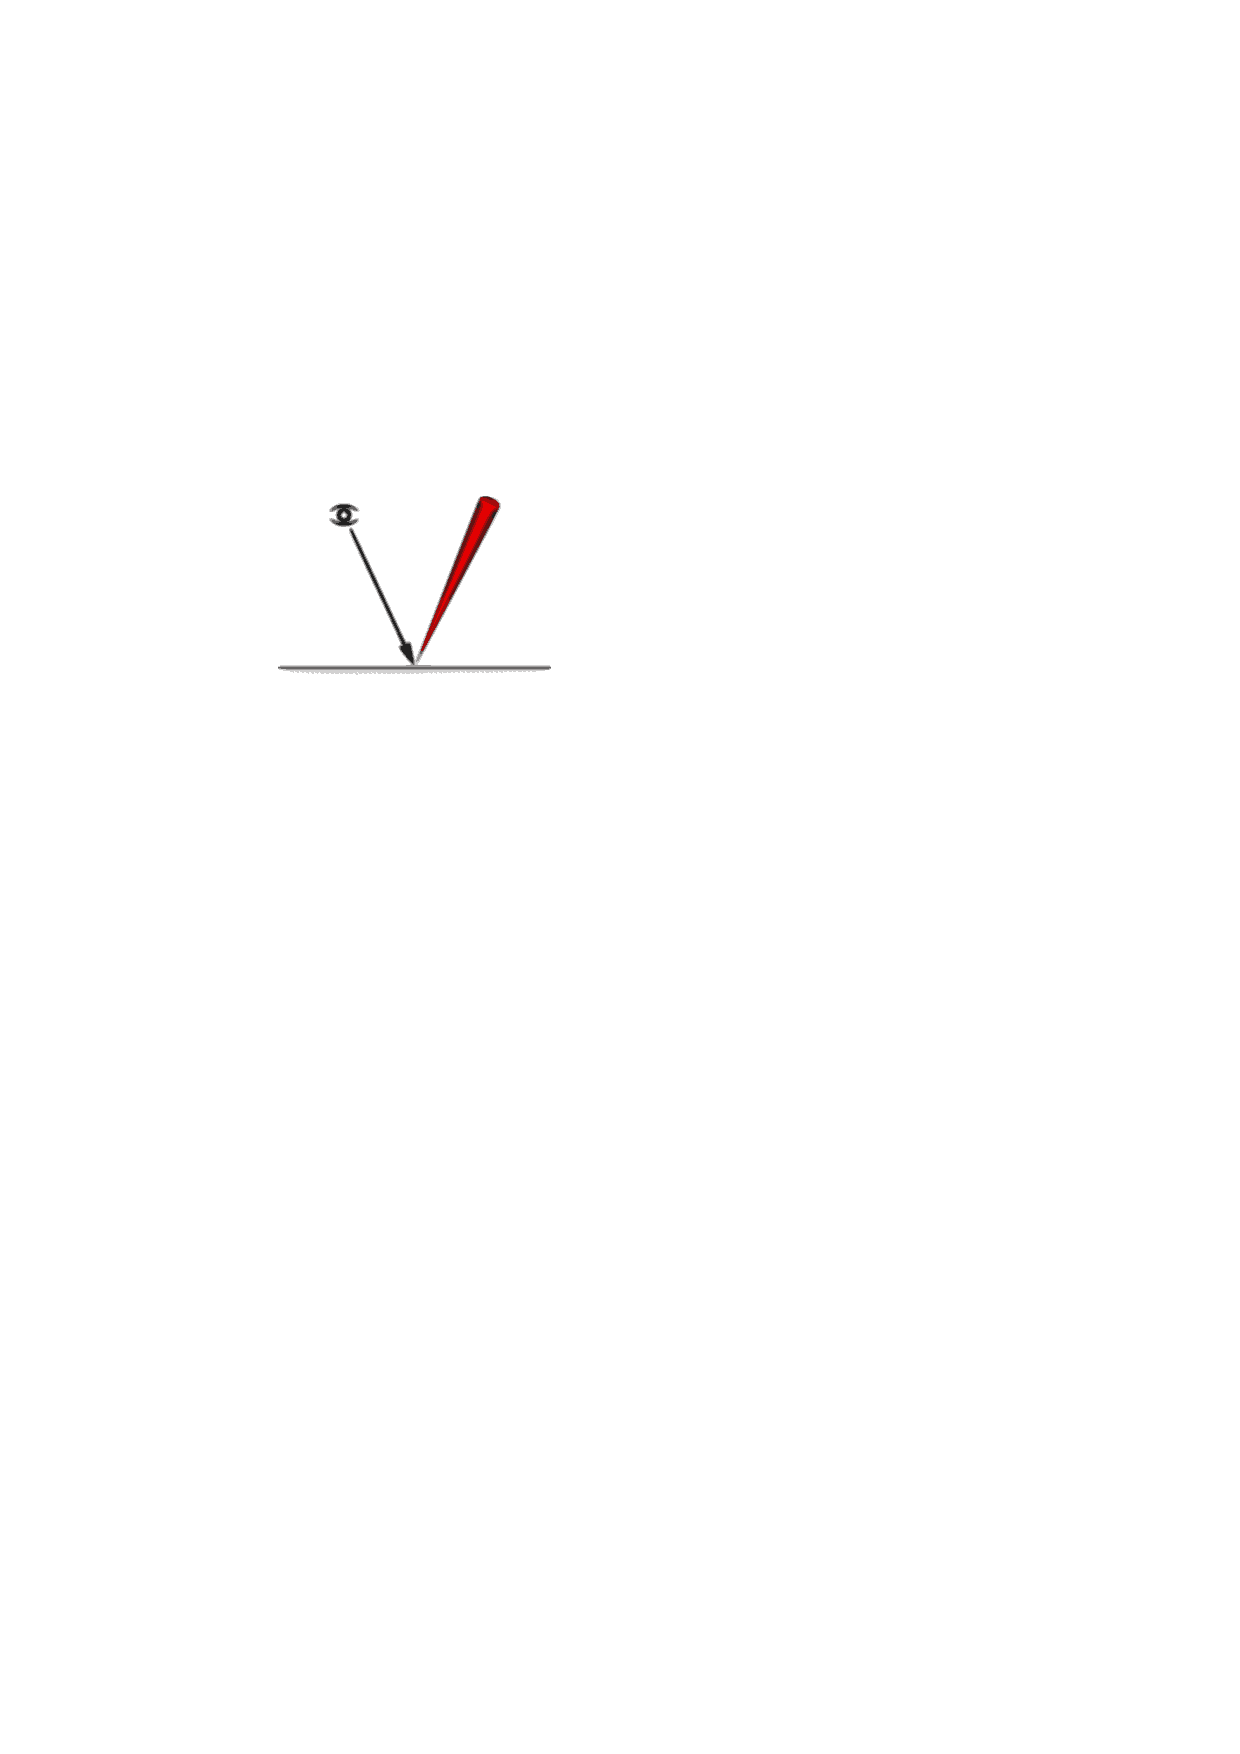
\includegraphics[width=\linewidth]{media/spec_cone.png}
		\caption*{Cono para el lóbulo especular.}
	\end{subfigure}\hfill
	\begin{subfigure}[t]{.33\linewidth}
		\centering
		\captionsetup{justification=centering}
		\includegraphics[width=\linewidth]{media/brdfallcone.png}
		\caption*{Discretización de la BRDF en conos.}
	\end{subfigure}
	\caption{Ilustración de la distribución de los conos utilizados para representar la \ac{BRDF} Blinn-Phong \cite{Oliver:2012:UEE:2341836.2341909}.}
	\label{fig:brdf_cones2}
\end{figure}

\subsection{Sombras Suaves} % (fold)
\label{sub:sombras_suaves_con_trazado_de_conos}
El trazado de conos contra vóxeles también puede xser utilizado para realizar pruebas de oclusión sobre una superficie. Para esto en nuestra implementación trazamos un cono desde la posición del fragmento en dirección opuesta a la dirección de la luz incidente. La apertura del cono permite modular el umbral de la sombra resultante. A mayor apertura más suave y esparcida es la sombra.

\begin{figure}[H]
	\centering
	\captionsetup{justification=centering}
	\includegraphics[width=.4\linewidth]{media/shadow_cone.pdf}
	\caption{Descripción gráfica del recorrido de un cono empleado para sombreado de superficies.}
\end{figure}

% subsection sombras_suaves_con_trazado_de_conos (end)
